\begin{figure}[!ht]
	\centering
	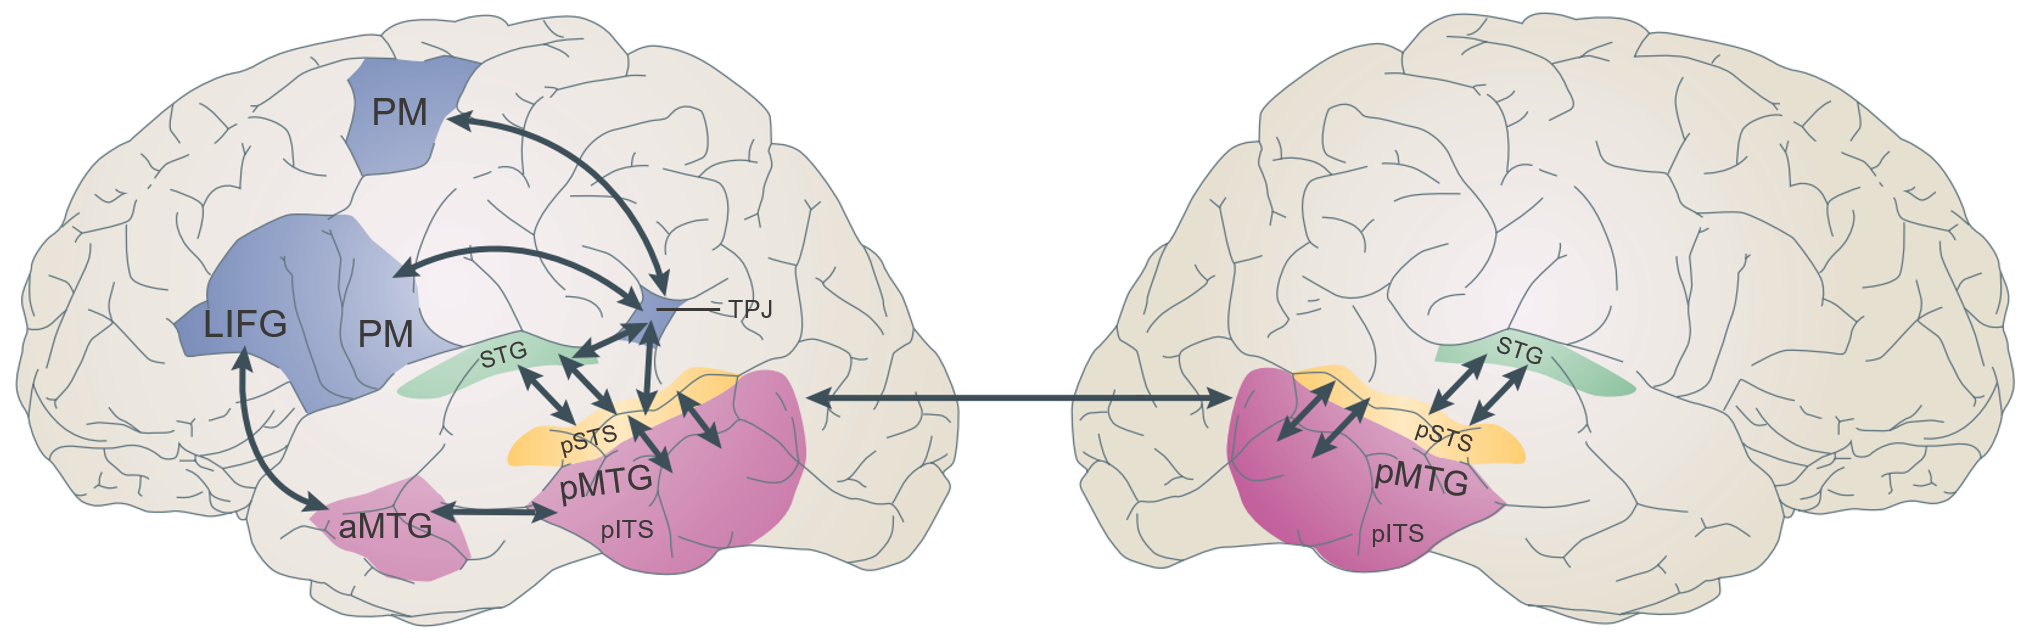
\includegraphics[width=.9\textwidth, clip=true]{./Chapters/01_Introduction/Images/Language_network_all_labels}
	\caption{Brain structures involved in language comprehension and production. Colors indicate different functional roles: pink = lexico-semantic interface, yellow = phonological network, green = spectrotemporal analysis of speech sounds, blue = articulatory network. LIFG = left inferior frontal gyrus, PM = premotor cortex, aMTG = anterior middle temporal gyrus, pMTG = posterior middle temporal gyrus, STG = superior temporal gyrus, TPJ = temporoparietal junction, pSTS = posterior superior temporal sulcus, pITS = posterior interior temporal sulcus. Figure adapted from \citet{hickok2007}}
    \vspace*{-10pt}
	\label{fig:language}
\end{figure}